\section{Conclusion and Discussion}
\label{sec:DiscConcl}
\subsection{Performance of Classifiers for both cases}
The performance of the classifiers for both cases, and their shortcomings, will be summarized in this section. \\
\subsubsection*{Case 1}
For Case 1, the recommended classifier is a Parzen density estimating classifier, combined using the product rule with a quadratic discriminant classifier which is applied to a dataset (representing the objects with pixels) whose dimensionality is reduced using principle component analysis preserving 90\% of the original variance. All provided data was used to train this classifier (10x1000=10,000 objects). The error rate was determined to be 0.0219 with standard deviation 5.3125e-4 using cross validation. The benchmark test yields an error rate of 0.0260.\\
Although this result is more than sufficient, some improvements could be made. In the interest of time, support vector machines were not considered in depth in this report, due to the long time it takes to calculate the classifier. According to the literature, they offer a promising prospect for classifying in high dimensional spaces, which would be a major advantage for this case since the pixel representation was used.
%When investigating scenario 1, PCA turned out to interfere dramatically with the performance of the Parzen classifier. This effect cannot be explained by the authors and warrants further research. \\
Furthermore, a brief look was given dissimilarity measures. Results were promising, but could not be pursued further in the interest of time. Testing the classifiers for different dissimilarity measures and using meticulously chosen prototypes might have improved the error rates, maybe beyond the results obtained using the pixel representation. \\

\subsubsection*{Case 2}
For Case 2, the recommended classifier is a Linear Discriminant classifier trained on the dissimilarity-representation dataset (using all objects as prototypes) that has its features reduced to 29 by means of PCA. 10 objects per class were used to train this classifier (100 objects) and the remaining 990 per class were used to test on. The error rate was determined to be 0.2184 with a standard deviation resulting from variation of the training set of 0.0153. The benchmark test (using \texttt{nist\_eval.m}) yields an error rate of 0.194\\
Although this result is sufficient, improvements could be made to make it more usable. One major improvement could be made by allowing the design to incorporate a set of prototypes, in stead of using the data in each batch. One could argue that this goes against the description for Case 2, but training will still involve each new batch. The major advantage of providing prototypes, is that they can be carefully selected to incorporate a wide variety of digits. This will yield a robust and versatile classifier. An alternative approach would be to incorporate a GUI, from which prototypes can be selected by hand for each batch. \\
Another point of interest in the design of Case 2, is the Support Vector classifier. For this classifier, only polynomial kernels were tried. Different kernels might have produced a different (better) result. Especially an advanced kernel like the ‘tangent distance kernel’, which incorporates rotation- and scaling insensitivity, could have improved the error rate.\\



\subsection{Usefulness of the pre-processing}
Finally, the image processing part of the presented algorithms needs to be evaluated. The classifiers for both cases were trained again, this time on a dataset without blob-removal and Gaussian smoothing (note that in case 1 there was also no blob-removing during the normal training, due to a large computation time.). The results are shown in table \ref{tab:improsconc}.
\begin{table}[H]
	\centering
	\caption{Estimated errors of the used classifiers for both cases, with and without the image processing.}
	\label{tab:improsconc}
	\begin{tabular}{l|l|ll}
		& Classifier                                                                                    & \begin{tabular}[c]{@{}l@{}}Error with \\ pre-processing\end{tabular} & \begin{tabular}[c]{@{}l@{}}Error without \\ pre-processing\end{tabular} \\ \hline
		Case 1 & \begin{tabular}[c]{@{}l@{}}Combination of ParzenC with QDC \\ (with PCA applied)\end{tabular} & 0.0219                                                               & 0.0309                                                                  \\
		Case 2 & LDC (with PCA applied)                                                                        & 0.2184                                                               & 0.2550                                                                 
	\end{tabular}
\end{table}
\noindent In both cases, implementation of the image processing makes the classifier perform better. In Case 1 this is only slightly better, and absence of the image processing still yields an error below the desired value, but in Case 2 the difference is larger. There, the absence of image processing results in a classifier performing worse than desired. \\
Some optimization could be done however. To start, the size of the images was chosen to be 16x16 pixels. This choice was motivated by the wish to reduce the run-times of the algorithms. The effect of using differently resized images for training could be investigated in the future. It seems logical that using larger, more detailed images, could improve classification up to a certain point. Similarly with the value for the Gauss filter: it was chosen to be 0.8 using visual inspection of the resulting images, but this value was not optimized considering the error rates of the classifiers. \\


\section{Recommendations}
\label{sec:recom}

When continuing designing the digit classification system for the purpose of classifying bank cheques, the following points are worth taking a closer look at. 
\begin{itemize}
	\item \textbf{Implement a reject option:} Especially when dealing with important interactions like bank cheques, any mistake made by the system may be a costly one. It is possible to lower the error rate further by implementing a reject option. This means that the system will abstain from making a definitive decision when the digit cannot be classified with a certainty above a certain threshold. After a digit is rejected several continuations are possible: the cheque containing a rejected digit can then be handled by human employees, or the submitter of the cheque can be contacted automatically, for example.	
	\item \textbf{Discontinue case 2 classification:} In case 2, a new classifier is trained for every batch of cheques to be processed. It seems difficult to come up with a real world scenario in which this would be an efficient procedure. A large training set containing handwritten digits is available, which makes it possible to create a classifier with an error rate below 3\%. This classifier can easily be used for all batches of cheques, without adaptation problems. To keep the classifier up to date with handwriting trends it can be retrained after a certain amount of time. 
	Training a new classifier for every batch delivers an error rate close to 20\%. Practically all submitted cheques would suffer misclassification in several digits. Discontinuation of this procedure should therefore be considered.
	
	\item \textbf{Investigate adding extra features:} The image analysis toolbox used in this report produces at most 14 usable features. This turned out to be insufficient to reach the thresholds set for the error rate. If the dimensionality of the feature space could be enlarged, this might benefit the performance of the classifiers (for case 1 in particular). Investigating ways to extract more features from the given images might turn out to be beneficial. Classifying using feature representation might be able to compete with the pixel data approach.
	\item \textbf{Investigate combining different representations:} The possibility to combine classifiers was considered in this report, but not the combination of different representations. For instance for Case 1, combining a classifier which is able to classify ‘8’ and ‘9’ using features or dissimilarities, with the classifiers described above using the pixel data approach, might further decrease the error rate. 
	\item \textbf{More training data?:} For scenario 2, using more training data would obviously help, but this is not in the spirit of this scenario. For scenario 1 a learning curve was made for the recommended combination of classifiers, which can be seen in figure \ref{fig:learning}. The apparent error sinks to zero, because the Parzen classifier gives an error of zero on its own training set. The estimated true error seems to converge to an asymptotic value. This suggests that the attained error will not decrease significantly after adding more training objects.
\begin{figure}[H]
	\centering
	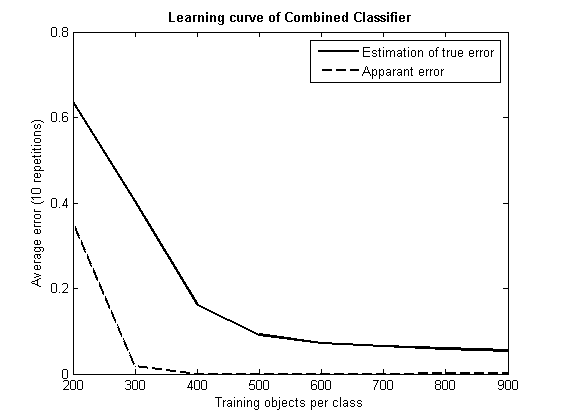
\includegraphics[scale=0.8]{images/pr_figure_5.png}
	\caption{Learning curve for the combined classifier of Case 1.}
	\label{fig:learning}
\end{figure}
	\item \textbf{Remarks about computation time}
	\begin{enumerate}
		\item \textit{Case 1:} For Case 1, once the classifier is trained on the entire dataset, time is not so much an issue. The training of the classifier itself takes a long time though. This is due to the large amount of data, in combination with the relatively cumbersome image processing algorithms in the pre-processing phase. If, for whatever reason, a new classifier has to be trained on a new datafile of numbers, this should be taken into account. \\
		If the classification itself needs to happen faster, for whatever reason, a (proper) implementation of an SVM might be preferred over ParzenC. While the training of an SVM might take long, its classification-performance after training is fast.
		\item \textit{Case 2:} In the instance of Case 2, more could be done to optimize the training of the classifier. Since the classifier is trained for each batch of cheques (and there will presumably be a lot of batches) this will benefit the user. Again, the most time-consuming factor here is the pre-processing. One way to optimize this (and by the way, this will also work for Case 1!) is to incorporate parallel computing in the algorithm, using \texttt{parfor} in stead of \texttt{for} loops. This will spread the calculations over the different cores of the computer, resulting in a much faster runtime.
	\end{enumerate}
\end{itemize}